\section{Evaluation}
\label{sec:eval}

% Jenny, feel free to modify this as you see fit
We tested our BiscuitSpy prototype on the an open home wireless LAN with MAC Address filtering as well as on the open Princeton University WiFi network, which also has MAC Address filtering. Due to factory configuration issues, we were never able to capture useful packets from devices on either network. However, we deem our current prototype sufficient for demonstrating the feasibility of profiling a user based on HTTP cookies.

Our results show that almost all cookies contain a unique browser identifier which can be used to pinpoint individual users. Furthermore we identified three main types of personal information that can be captured through cookies:

\begin{enumerate} \itemsep1pt \parskip0pt \parsep0pt
  \item Browsing habits are leaked through timestamps
  \item Location information is leaked in cookies
  \item Username and e-mail are leaked in cookies
\end{enumerate}

\subsection{Leaking of browsing habits}
The \_utma cookie is one of the most prevalent cookies and is used by BiscuitSpy to create a profile of the user's browsing habits. For any website the user visits that contains this cookie BiscuitSpy can determine the initial visit time to that website, the most recent visit time, the current visit time and the number of visits. Especially the intial visit combined with the number of visits allows us to infer how long the user has at least used the current browser and whether he regularly visits the website. The example in figure ~\ref{fig:utma2} is taken from the author's \_utma cookie of  \url{www.github.com}.

\begin{figure}[h]
\centering
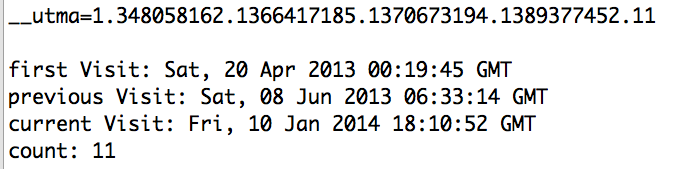
\includegraphics[scale=0.4]{./diagrams/utma2.png}
\caption{utma cookie with parsed timestamp information}
\label{fig:utma2}
\end{figure}


\subsection{Leaking of location information}
We also discovered that certain cookies leak very detailed geographical information. For example \url{http://www.washingtonpost.com/} contains a \texttt{rpld1} cookie that tells us that the user is accessing the website through a \texttt{princeton.edu} network, that he is located in Princeton, New Jersey and even passes the longitude and latitude of his current location in plaintext!

\begin{figure}[h]
\centering
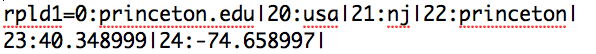
\includegraphics[scale=0.5]{./diagrams/location.png}
\caption{rpld1 cookie from washingtonpost.com leaking location information}
\label{fig:location}
\end{figure}


\subsection{Leaking of username and e-mail}

While examining cookie data captured from BiscuitSpy we came across a particularly disturbing cookie from wordpress.com called \texttt{wpc\_wpc}
\begin{figure}[h]
\centering
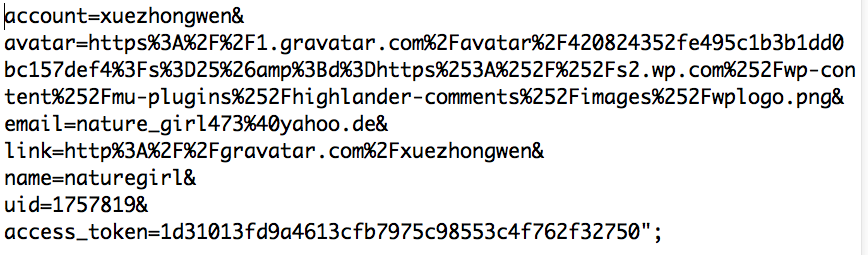
\includegraphics[scale=0.4]{./diagrams/wpc.png}
\caption{wpc\_wpc cookie from wordpress.com leaking username and e-mail}
\label{fig:wpc}
\end{figure}

 This cookie transmitted the username and e-mail in plaintext and was present on all websites that are based on wordpress.com. For example a visit to the website \url{http://www.hustlermoneyblog.com} transmits the cookie as seen in figure ~\ref{fig:wpc} which contains the user's email address, username and user id.
\\
\\
The above three types of user data leaks allow BiscuitSpy to create a user profile that contains his browsing habits, location information and username and e-mail. In addition BiscuitSpy will also collect unique browser identifier cookies to be able to cross reference visits to different websites and recognize users in a new browsing session.

\subsection{Cookies on Alexa Top 10 websites}

In addition to determining particularly critical user data leaks that can be used to profile a user, we also looked at the top 10 websites as determined by Alexa and examined their cookie usage. We only focused on the English websites out of the top 10 websites (excluding the 3 Chinese websites baidu.com, qq.com and taobao.com) and were specifically interested in what fraction of them uses the cookies as described in paragraph ~\ref{sec:background} and used by BiscuitSpy for profiling.

\begin{table}[h]
\centering

\begin{center}
    \begin{tabular}{ | l | p{6cm} | p{6cm} |}
    \hline
    Website & own domain cookies & third party cookies \\ \hline

google.com & 8 cookies including PREF and SID & none \\ \hline
facebook.com & 12 cookies including 'datr' & none \\ \hline
youtube.com & 9 cookies & doubleclick 'id', google PREF and SID \\ \hline
yahoo.com & 19 cookies & none \\ \hline
wikipedia.org & 4 cookies & none \\ \hline
amazon.com & 9 cookies including apn-user-id & doubleclick 'id' \\ \hline
live.com & 9 cookies & none \\ \hline

    \end{tabular}
\end{center}

\caption{Cookie usage on English websites from Alexa Top 10 websites}
\label{tab:alexa}

\end{table}


In general, we see from Table ~\ref{tab:alexa} that these websites tend to rely on their own cookies.
Only two websites have the doubleclick 'id' cookie and the Google PREF cookie as third party cookies. It is also notable that wikipedia uses the fewest cookies, with 0 cookies on their start page \url{http://www.wikipedia.org} and only 4 cookies on their main page \url{http://en.wikipedia.org/wiki/Main_Page}
